\documentclass[11pt]{beamer}
\usetheme{Warsaw}
\usepackage[utf8]{inputenc}
\usepackage[german]{babel}
\usepackage[T1]{fontenc}
\usepackage{amsmath}
\usepackage{amsfonts}
\usepackage{amssymb}
\usepackage{graphicx}
%\author{}
%\title{}
%\setbeamercovered{transparent} 
%\setbeamertemplate{navigation symbols}{} 
%\logo{} 
%\institute{} 
%\date{} 
%\subject{} 
\begin{document}

%\begin{frame}
%\titlepage
%\end{frame}

%\begin{frame}
%\tableofcontents
%\end{frame}

\begin{frame}{Kondensator - Cassy - Beschreibung}
- gleicher Aufbau wie bei der Messung mit dem Oszilloskop\\
- Auswertung der Daten mit Python\\
- Vergleich mit Herstellerangaben\\
\end{frame}

\begin{frame}{Kondensator - Cassy - Aufbau}
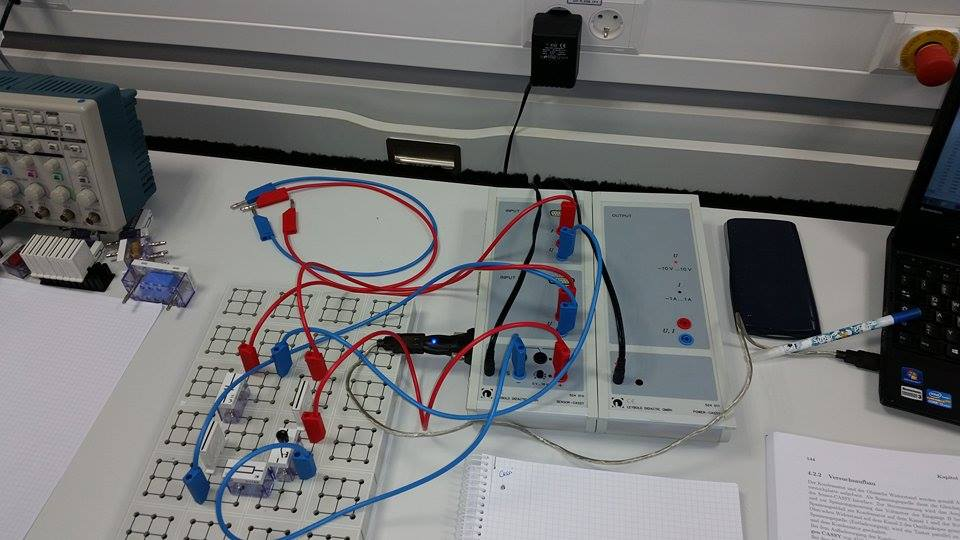
\includegraphics[scale=0.2]{12834837_1207198225971904_686312351_n.jpg}
\end{frame}

\begin{frame}{Kondensator - Cassy - Rohdaten}
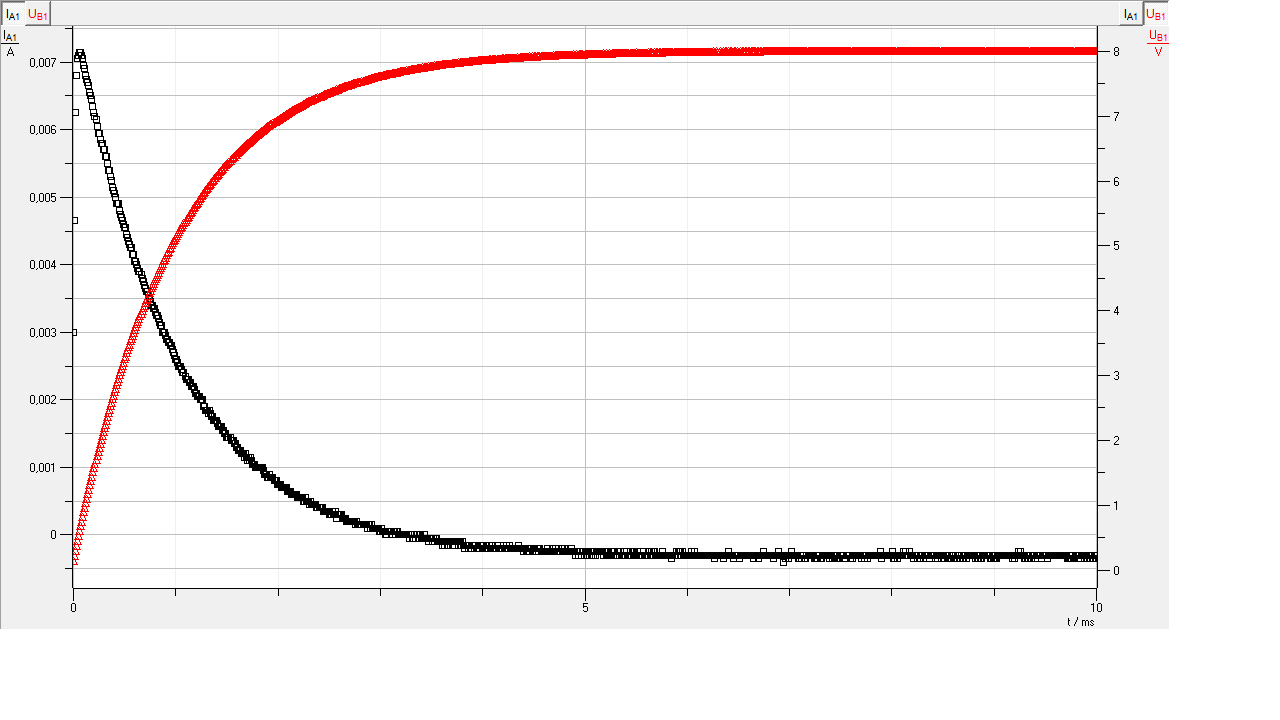
\includegraphics[scale=0.2]{auf1.png}\\
Aufladevorgang (U in V [rot], I in A [schwarz]gegen t in ms)
\end{frame}

\begin{frame}{Kondensator - Cassy - Rohdaten}
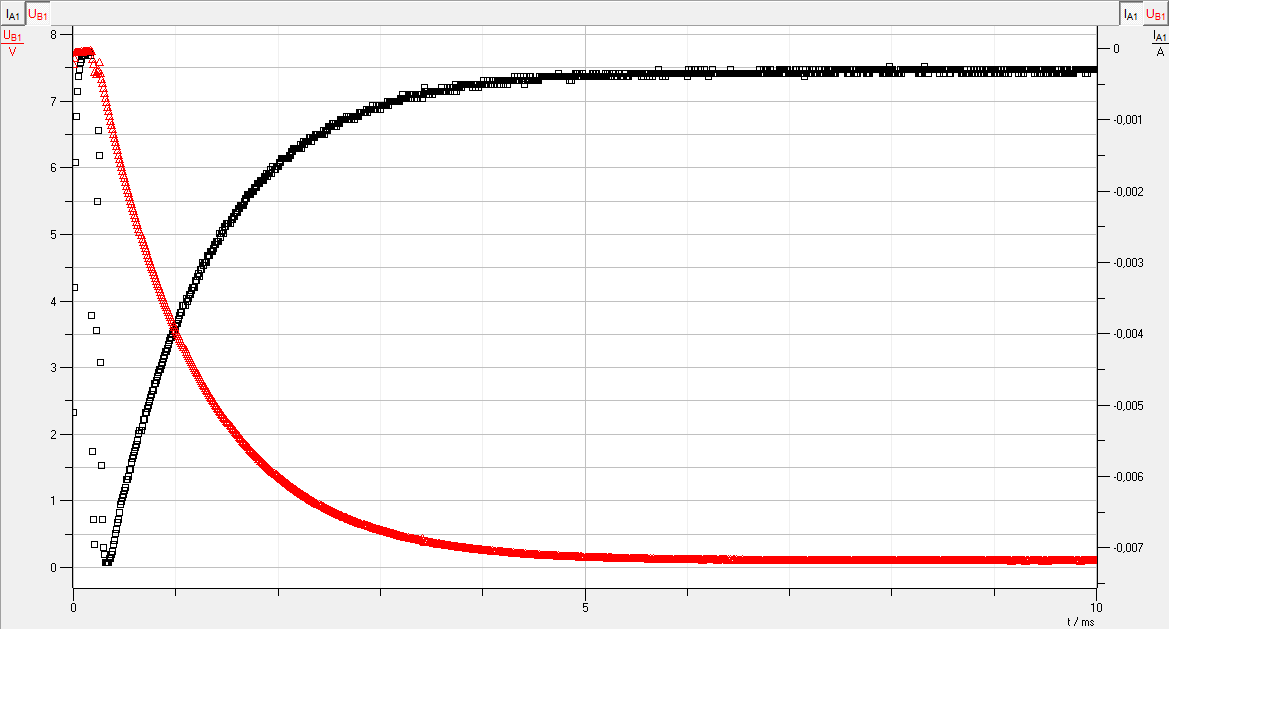
\includegraphics[scale=0.2]{ent1.png}\\
Entladevorgang (U in V [rot], I in A [schwarz]gegen t in ms)\\
\end{frame}

\begin{frame}{Kondensator - Cassy - Verarbeitung - Übersicht}
\begin{itemize}
\item Offsets über Cassy grafisch bestimmen
\item Daten logarithmieren
\item eine Gerade an die Datenpunkte fitten mittels Linearer Regression
\item Residuum bilden
\item Fit bewerten
\item gewichteten Mittelwert bilden
\end{itemize}
\end{frame}

\begin{frame}{Kondensator - Cassy - Beispiel}
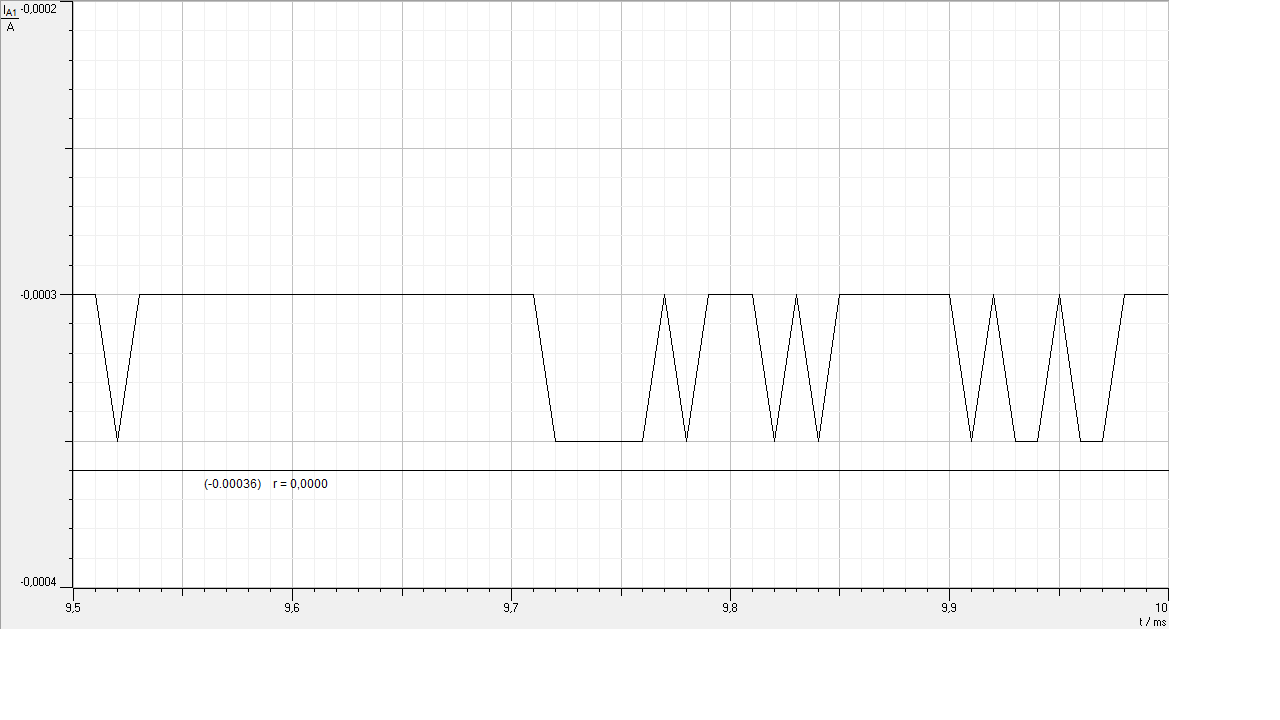
\includegraphics[scale=0.2]{offset_und_fehler.png}\\
\begin{itemize}
\item Offset und Ablesefehlerbestimmung
\end{itemize}
\end{frame}

\begin{frame}{Kondensator - Cassy - Beispiel}
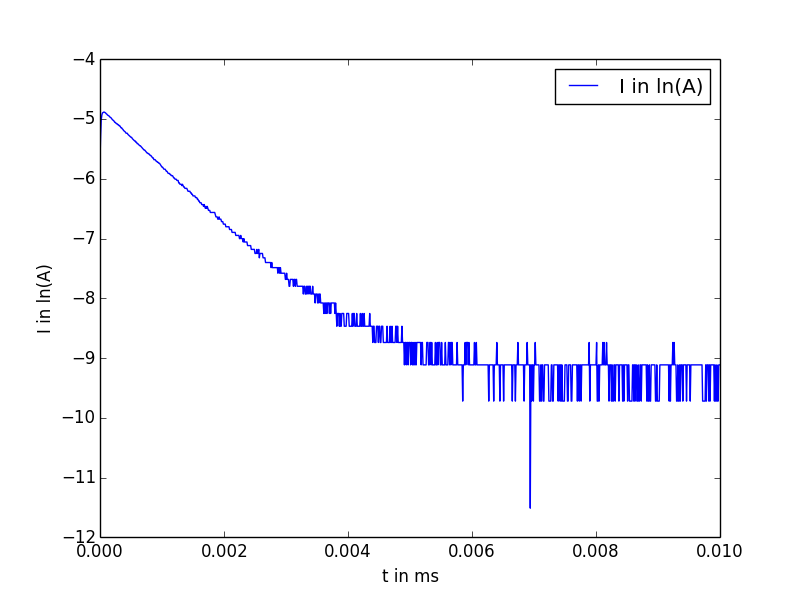
\includegraphics[scale=0.35]{ln(I)ggt.png}\\
Logarithmierter I-Datensatz (Einheiten siehe Grafik)\\
- Bereiche am Anfang und Ende werden nicht berücksichtigt
\end{frame}

\begin{frame}{Kondensator - Cassy - Beispiel}
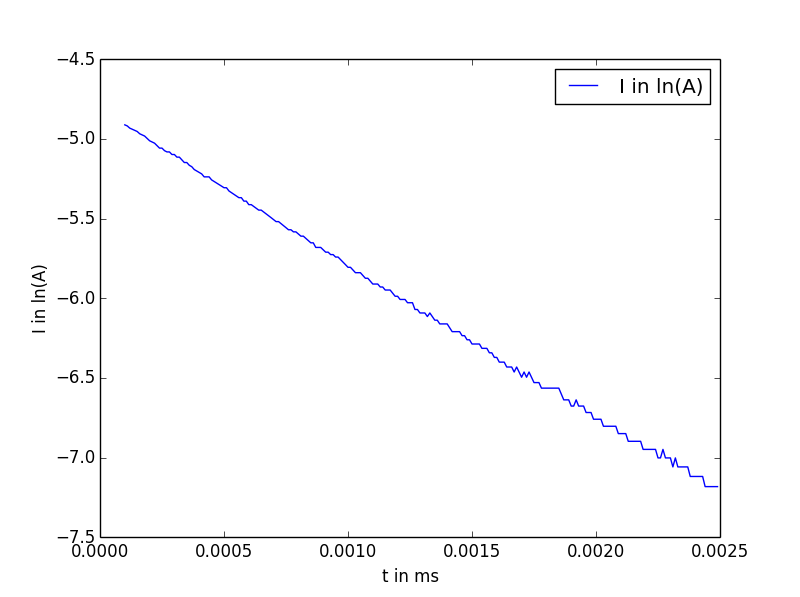
\includegraphics[scale=0.2]{ln(Ik)ggt.png}\\
Logarithmierter I-Datensatz mit angepasstem Bereich(Einheiten siehe Grafik)\\
- sieht nach einer Geraden aus\\
- Lineare Regression durchführen\\
\end{frame}

\begin{frame}{Kondensator - Cassy - Beispiel}
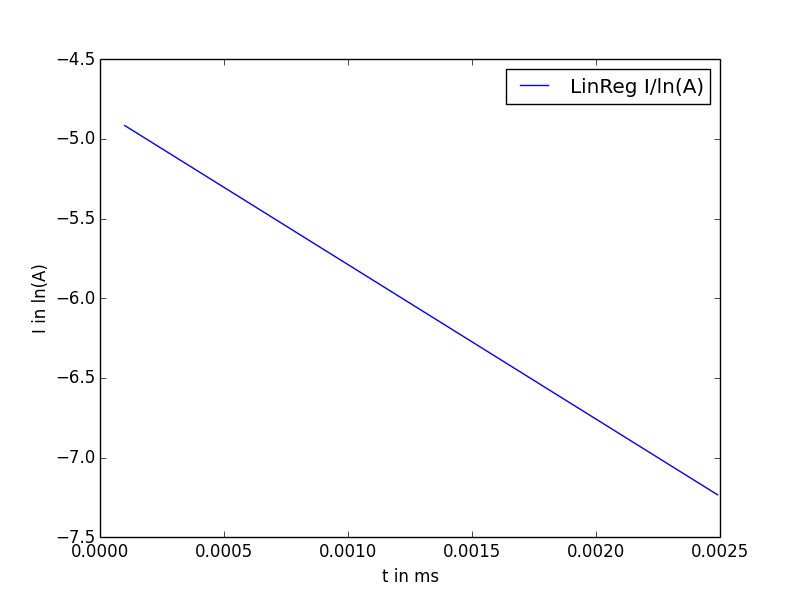
\includegraphics[scale=0.2]{lin_reg_I}\\
$\chi^2 = 3.046431$
\begin{itemize}
\item $a = -969.523$
\item $C = -\frac{1}{a\cdot R}$
\end{itemize}
\end{frame}

\begin{frame}{Kondensator - Cassy - Auswertung}
\includegraphics[scale=0.2]{residuum_I}\\
Residuum für I 
\end{frame}

\begin{frame}{Kondensator - Cassy - Auswertung}
\begin{itemize}
\item Fortpflanzung systematischer Fehler:
\begin{equation}
\sigma_{c_{sys}} = \frac{1}{a\cdot R^2}\cdot\sigma_{R_{sys}}
\end{equation}
\item gewichteten Mittelwert bilden:
\begin{equation}
\bar{C} = \frac{\sum{\frac{C}{(\sigma_{sys}+\sigma_{stat})^2}}}{\sum{\frac{1}{(\sigma_{sys}+\sigma_{stat})^2}}}
\end{equation}
\begin{equation}
\sigma_{C_{ges}} = \sqrt{\frac{1}{\sum{\frac{1}{(\sigma_{sys}+\sigma_{stat})^2}}}}
\end{equation}
\end{itemize}
\end{frame}

\begin{frame}{Kondensator - Cassy - Auswertung}
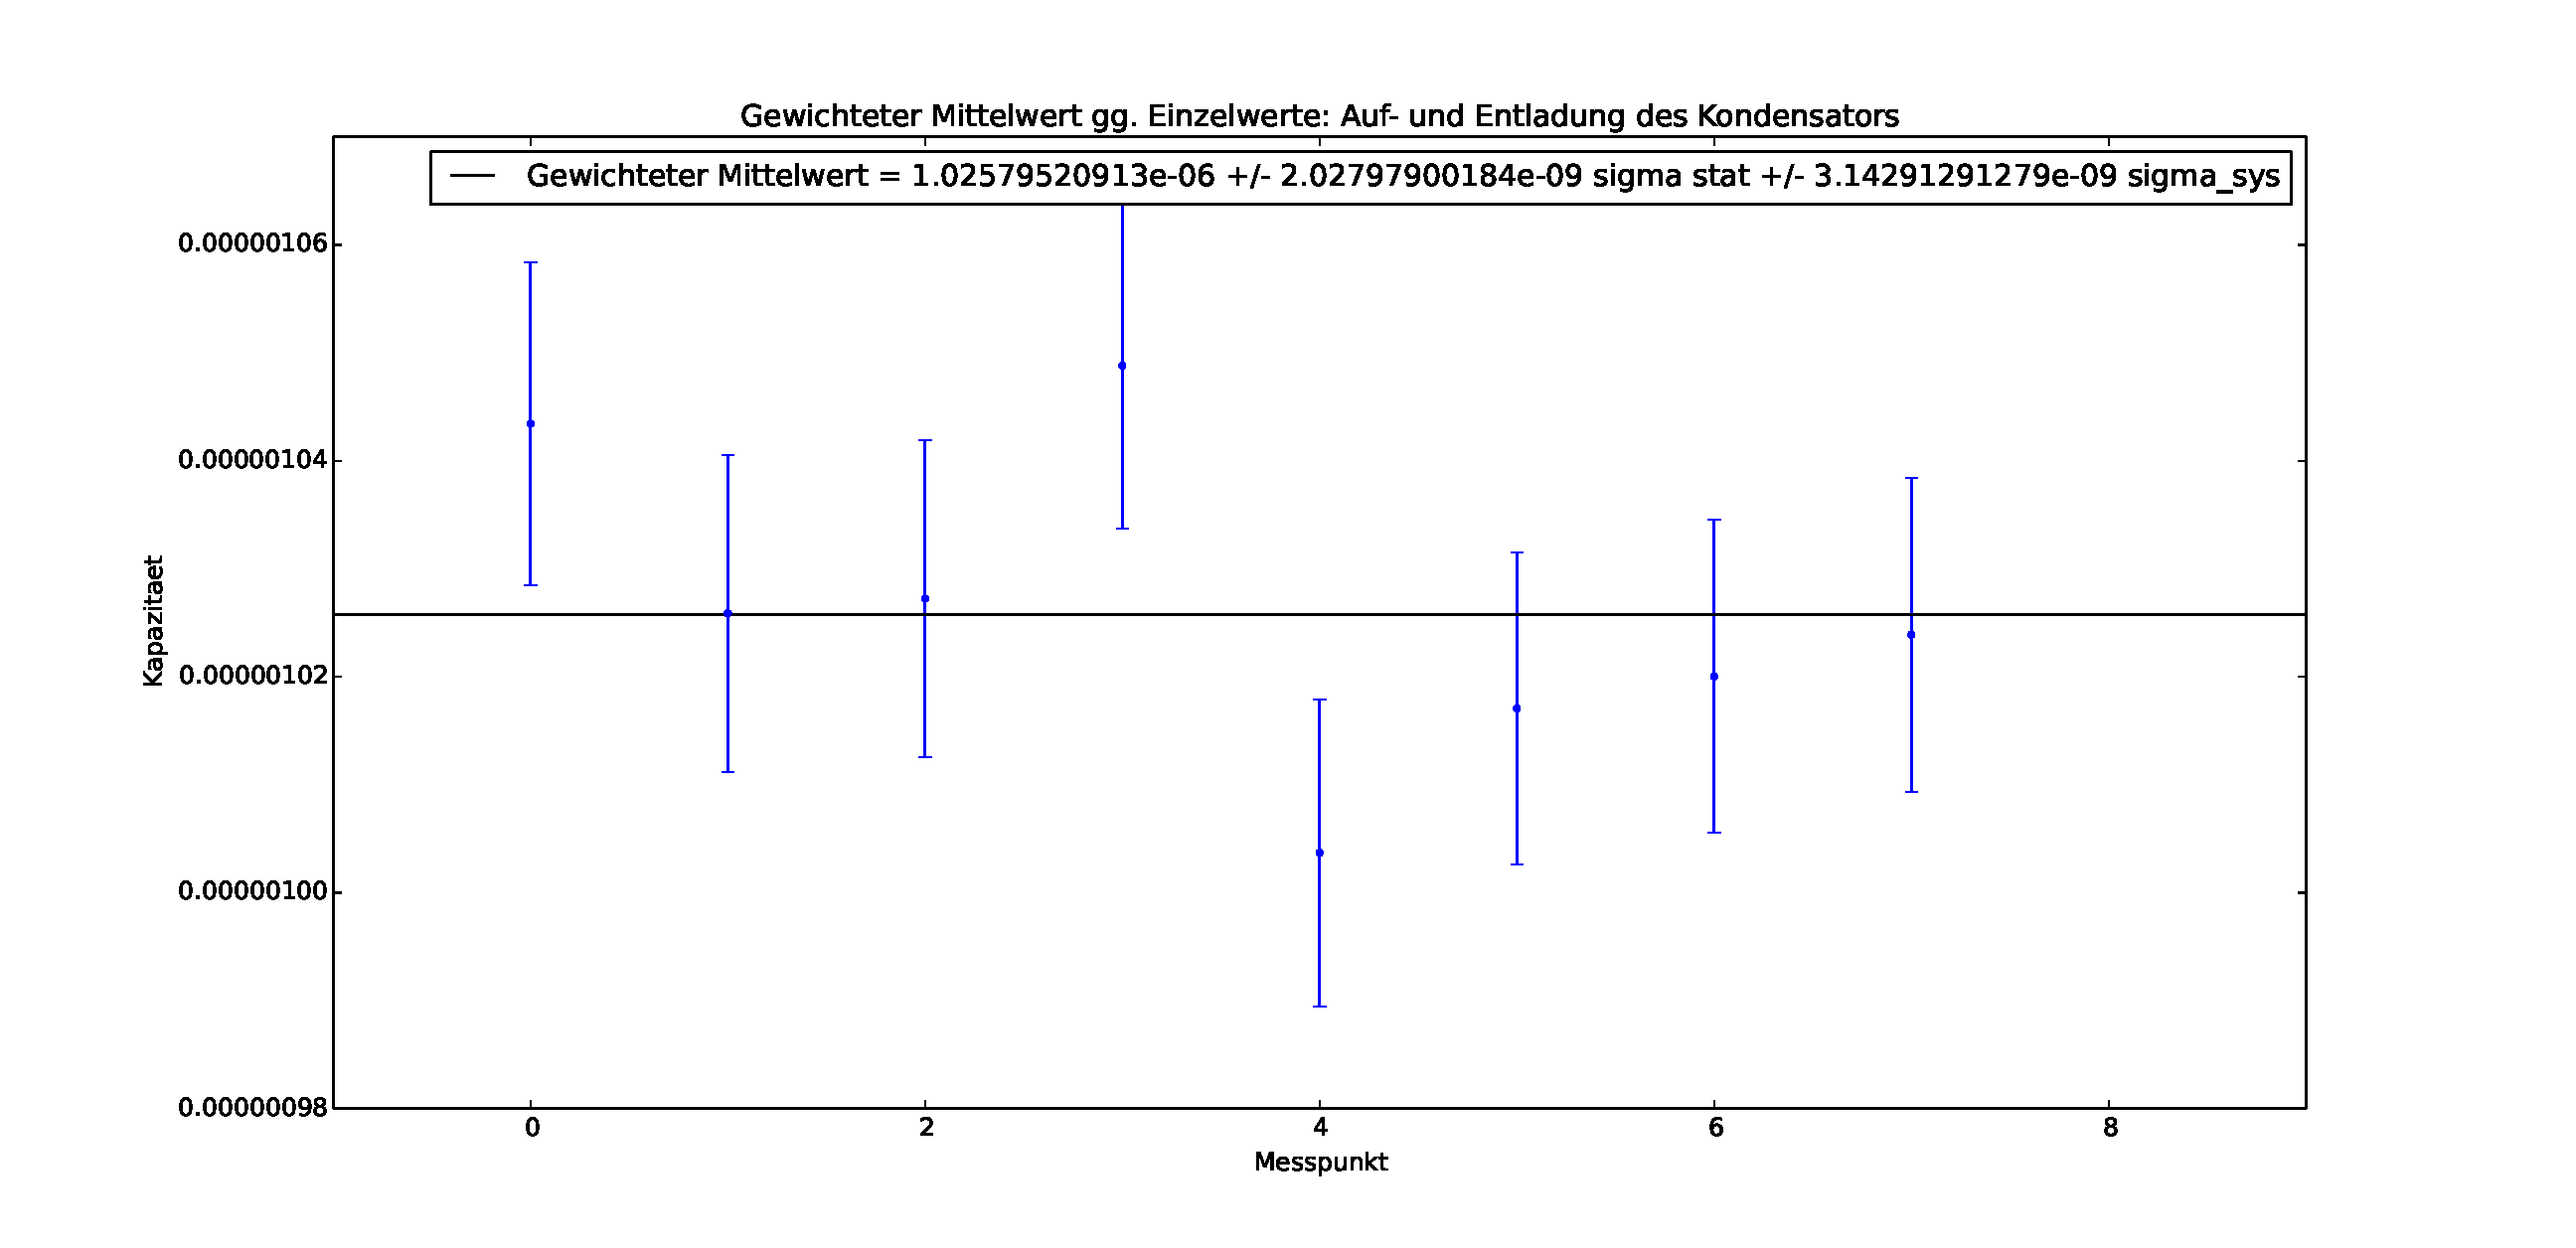
\includegraphics[scale=0.2]{verteilung_mean.eps}\\
- 60\% der Daten schneiden den Mittelwert mit ihren Fehlerbalken
\end{frame}

\begin{frame}{Kondensator - Cassy - Fazit}
\begin{itemize}
\item Kapazität-Endergebnis:
\begin{equation}
C = 1.026\mu F \pm 2.028\cdot 10^{-3}\mu F \pm 3.143\cdot 10^{-3}\mu F
\end{equation}
\item liegt innerhalb der 5\% Toleranzgrenze des Herstellers (0.95$\mu F$-1.05$\mu F$)
\begin{equation} \chi^2 = 3.046 
\end{equation} 
\item Wert stimmt mit Messung der Greenbox überein (0.999$\mu F \pm$0,25\%$\mu F$).

\end{itemize}
\end{frame}
\end{document}